% !TEX root = ../Report.tex

Since hardware specifications and computational power increased dramatically in the last years computational expensive machine learning approaches can be applied in various disciplines today. Progress in research on convolutional neural networks (CNN) has made it a very powerful tool for image processing.\newline
One challenging application is medical image computing (MIC). The main goal of MIC is to extract clinically relevant information from medical images. Segmentation is the process of delineating an image into meaningful segments (e.g. organs, bones, ...).\newline
In this project the goal was to segment the lungs of a human body from computed tomography (CT) scans of the chest from the LUNA16 dataset \cite{luna}. Every CT scan consists of a variable number of greyscale image slices in the axial, sagittal, and coronal anatomy planes. Given these slices a 3D model of the lung needs to be created. To reach this goal every slice of the CT scan was evaluated by a CNN architecture and a corresponding segmentation in the form of a label map for the lung and the bronchus on these slices was predicted. From these label maps a 3D model of the structure can be created. \newline

\begin{figure}[h!]
	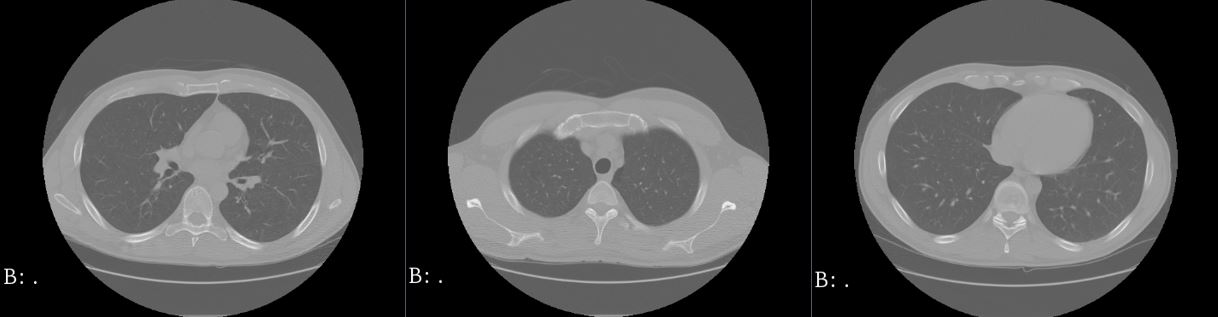
\includegraphics[width=0.49\textwidth, angle=0]{files/ctscans.jpg}
	\caption{CT scan from the LUNA16 dataset}
	\label{scan_picture}
\end{figure}

The segmentation of the lungs from the rest of the volume is the first step for further image processing. In the LUNA16 dataset problem statement the final goal is to detect nodules of the lung indicating cancer. The results from machine learning approaches can be a powerful support for doctors who treat patients with suspected cancer. The algorithms can reduce human errors, and may improve cancer detection rates. This could have a positive effect on health care quality and costs.\newline
In this work two different neural networks were trained and tested to segment the lung on the LUNA16 dataset. The networks were also examined and compared using a variety of metrics seen frequently in image processing literature.\newline
First a short overview on the DeepMedic and the U-Net architecture will be given and the work will be related to other traditional approaches for medical image segmentation. After that the process and implementation will be explained and then the results of the two algorithms will be examined and compared. A conclusion on the work will be drawn and future work outlined.
